\cotefile{156-4}

\scanpage{65}\mspage{64}
Inversement, donnons nous, \deleted{$\unsure{F_i\in|F_i}$} $\unsure{(}\forall i\in I)$ un $F_i\in\mathcal F_i$, quand peut-on dire qu'il existe $F\in\mathcal F$ telle que $\forall i$, $F_i$ soit la $i$ composante de $\deleted{\unsure{\mathcal F}}\unsure{F_0|F}$ ?

Déjà, il le faudrait pour \unsure{le|les} cas où tous les $F_i$ sauf un nb fini sont \deleted{$\varnothing$} vides. On va supposer donc

\uline{$C4$} Si $x,y\in M$ appartiennent à des comp connexes disjointes de $M$, alors $x$ et $y$ sont compatibles.

\deleted{Cor} \inserted{C'est néc et suffisant pour la \unsure{validité|\deleted{val}idité} des}

\uline{Corollaire 1} L'image de $\mathcal F\to\prod\mathcal F_i$ contient les $(F_i)_{i\in I}$ tels que $F_i=\varnothing$ \deleted{sauf} pour \deleted{\unsure{pres}} que tout $i$.

% The added Cor. 2 and its open angular enclosure stand to the right of Corollaire 1's final line.
% The lower-left arm of the enclosure points toward the continuation "est une bijection".
\figure{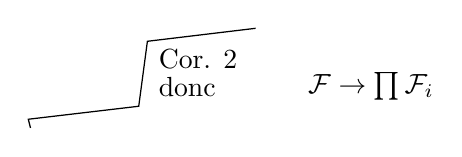
\begin{tikzpicture}[x=0.55cm,y=0.55cm]
\draw[line width=0.45pt] (-2.5,-1.4) -- (-2.55,-1.2) -- (0,-0.9) -- (0.2,0.6) -- (2.7,0.9);
\node[anchor=west,inner sep=0pt] at (0.45,0.2) {\inserted{\uline{Cor. 2}}};
\node[anchor=west,inner sep=0pt] at (0.45,-0.45) {\deleted{\unsure{donc}}};
\node[anchor=west,inner sep=0pt] at (3.9,-0.45) {$\mathcal F\to\prod\mathcal F_i$};
\end{tikzpicture}}
est une bijection dans \unsure{le\deleted{s}|les} \deleted{deux} cas où \deleted{suivants} \inserted{$I$ est fini.}

\deleted{a) $I$ est fini}

\deleted{b) Toute figure est de t.f. -- alors}

\uline{Cor 3} Supposons que les figures \deleted{\unsure{de|des}} $\in\mathcal F$ soient de t.f. \deleted{Alors il} \inserted{(resp. finies)}. Alors il en est de $=$ \deleted{\unsure{de}} pour $\mathcal F_i$, de plus $\mathcal F\unsure{\text{---}|\longrightarrow}\prod\mathcal F_i$ a comme image l'ens des $(F_i)$ tels que $F_i$ soit $\varnothing$ pour \unsure{pres|près|prés} que tout $i$.

\scanpage{66}\mspage{65}
Ceci résulte du \deleted{\uline{C}4 et} cor. 1 et du

\uline{Lemme} Pour que $F$ soit de t. f.\inserted{(resp. fini)} il f et s que a) les $F_i$ le soient et b) Tous les $F_i$ sauf un nb fini sont $\varnothing$.

Notations $\pi_0(F)$ (NB Si $F\leq G$ on a $\pi_0(F)\longrightarrow\pi_0(G)$\deleted{\unsure{)}}, et transitivité) $\pi_0(M)$, $\pi_0^{\substack{\deleted{\unsure{\mathrm{cat}|\mathrm{act}}}\\!}}(\unsure{.}\mathcal F)$. (\unsure{Attention}, le $\pi_0^{\unsure{\underset{\circ}{d}|!}}(\mathcal F)$ n'est pas le $\pi_0(F,\leq)$, mais le $\pi_0$ ``en tenant compte \unsure{du|des} Sup''. Si
% The tuple and its two interlinear glosses are reproduced together with their drawn pointers.
\figure{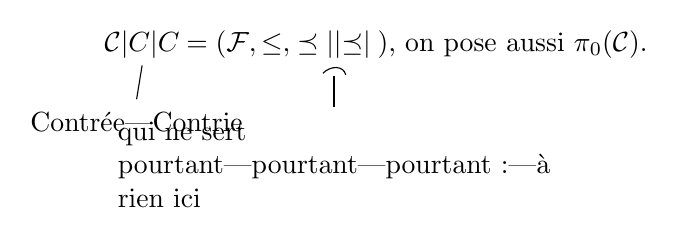
\begin{tikzpicture}[every node/.style={inner sep=1pt}]
  \node[anchor=base west] (initial) at (0,0) {$\unsure{\mathcal C|\mathscr C|C}$};
  \node[anchor=base west] (prefix) at (initial.base east) {$=(\mathcal F,\leq,$};
  \node[anchor=base west] (relation) at (prefix.base east) {$\unsure{\preceq|\leqslant|\deleted{\preceq}|\deleted{\leqslant}}$};
  \node[anchor=base west] (rest) at (relation.base east) {$)$, on pose aussi $\pi_0(\mathcal C)$.};
  \draw[thin] (initial.south) ++(0,-0.05) -- ++(-0.07,-0.43);
  \path (initial.south) ++(-0.07,-0.60)
    node[anchor=north] {\unsure{Contrée|Contrie}};
  \draw[thin] (relation.south) ++(0,-0.58) -- ++(0,0.40);
  \draw[thin] (relation.south) ++(-0.14,-0.15)
    .. controls +(0.10,0.10) and +(-0.03,0.12) .. ++(0.29,-0.02);
  \path (relation.south) ++(0,-0.73)
    node[anchor=north,align=left] {qui ne sert\\\unsure{pourtant|pour\deleted{tant}|\deleted{pourtant}} \unsure{:|à}\\rien ici};
\end{tikzpicture}}

Axiome renforcé

\uuline{C4 bis} Pour tout $(F_i)_i\in\prod\mathcal F_i$, $\deleted{\exists\mathcal F}$ $\exists F\in\mathcal F$ telle que $F\mid M_i=\unsure{F_i|\deleted{\mathcal F}F_i}$ pour $i\vdash I$,

\uline{\unsure{Contrée|Contrie} résiduelle} \uline{Support} \uline{et} \uline{cosupport}

Soit $\deleted{\unsure{(F_i)\in\mathcal F|(H_i)\in\mathcal F}}$ $\Phi\subset\mathcal F$ un ens. de
% The inserted H_i is connected to the position after figures by a long oblique stroke.
\figure{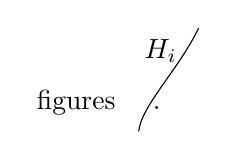
\begin{tikzpicture}[x=1cm,y=1cm]
  \node[anchor=base east] at (0,0) {figures};
  \node[anchor=base] at (0.45,0.65) {\inserted{$H_i$}};
  \draw (0.17,-0.28) .. controls (0.20,0.04) and (0.68,0.51) .. (0.93,1.03);
  \node[anchor=base] at (0.40,0) {.};
\end{tikzpicture}}
\deleted{On posera} Soit $F$ une figure. Pour \deleted{Cosupp. $\Phi$} que $F$ soit \unsure{disjointe|disjoint} de tous les $H_i$, il f et s. que ce soit le cas pour toutes les \unsure{strates} de $F$ (à cause de C3). \deleted{Posons} Posons

\scanpage{67}\mspage{66}
% The raised inclusion and the long connecting stroke below the second row
% are reproduced with their formula labels; the labels occur only here.
\figure{
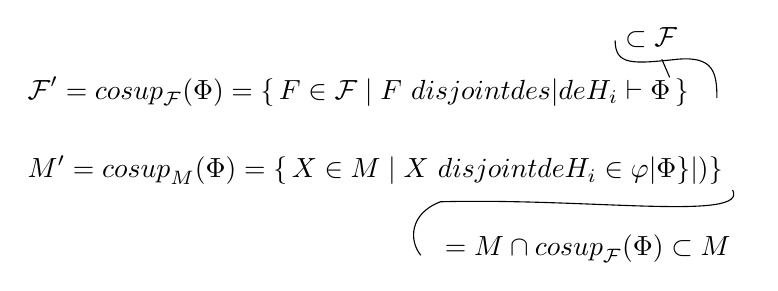
\begin{tikzpicture}[x=1cm,y=1cm,every node/.style={inner sep=0pt}]
  \node[anchor=west] (top) at (0,0) {$\displaystyle
    \mathcal F'=\operatorname{cosup}_{\mathcal F}(\Phi)
    =\{\,F\in\mathcal F\mid F\ \text{disjoint \unsure{des|de} }H_i\vdash\Phi\,\}$};
  \node[anchor=south east] (addition) at ([xshift=-.15cm,yshift=.55cm]top.east)
    {$\inserted{\subset\mathcal F}$};
  \draw ([xshift=-.12cm,yshift=.1cm]addition.south west)
    .. controls ([xshift=-.12cm,yshift=-.22cm]addition.south west)
    and ([xshift=.1cm,yshift=-.2cm]addition.south west)
    .. ([yshift=-.14cm]addition.south east)
    .. controls ([xshift=.45cm,yshift=-.1cm]addition.south east)
    and ([xshift=.35cm,yshift=.25cm]top.east)
    .. ([xshift=.35cm,yshift=-.08cm]top.east);
  \draw ([xshift=-.2cm,yshift=-.14cm]addition.south east)
    -- ([xshift=-.25cm,yshift=.18cm]top.east);
  \node[anchor=west] (second) at (0,-1) {$\displaystyle
    M'=\operatorname{cosup}_{M}(\Phi)
    =\{\,X\in M\mid X\ \text{disjoint de }H_i\in
    \unsure{\varphi|\Phi}\unsure{\rbrace|)\rbrace}$};
  \node[anchor=west] (third) at (5.3,-2) {$\displaystyle
    \inserted{=M\cap\operatorname{cosup}_{\mathcal F}(\Phi)\subset M}$};
  \draw ([xshift=.12cm,yshift=-.25cm]second.east)
    .. controls ([xshift=.33cm,yshift=-.65cm]second.east)
    and ([xshift=-1.8cm,yshift=.65cm]third.east)
    .. ([xshift=-.05cm,yshift=.6cm]third.west)
    .. controls ([xshift=-.45cm,yshift=.45cm]third.west)
    and ([xshift=-.45cm,yshift=.1cm]third.west)
    .. ([xshift=-.3cm,yshift=-.08cm]third.west);
\end{tikzpicture}}

\deleted{Donc \unsure{on aura|on a}, pour $F\in\mathcal F$ posant $\mathcal F'=\operatorname{cosup}_{\mathcal F}$,}

\[
\begin{aligned}
&\deleted{\unsure{\phi|\Phi}}\qquad
\deleted{\mathcal F'=\operatorname{cosupp}_{\mathcal F}(\Phi),\quad M'=\mathcal F'\cap M,}\\[-2pt]
&\qquad\deleted{F\in\operatorname{cosup}_{\unsure{,|\mathcal F}}}
\qquad\qquad\deleted{=\operatorname{cosup}_{\deleted{\unsure{\mathcal F}}M}(\mathcal F)}
\end{aligned}
\]

Donc pour $F\in\mathcal F$

% Slanted left marginal note, the brace display, and the right marginal
% note are one graphical group. Neither margin text is duplicated.
\figure{%
\begin{tikzpicture}[x=1cm,y=1cm,every node/.style={font=\small}]
\node[anchor=west] (brace) at (4.0,0) {$\displaystyle
\left\{\begin{aligned}
F\in\mathcal F'&\Longleftrightarrow\overline F\subset M'\\
M'&=.\mathcal F'\cap M
\end{aligned}\right.$};
\node[anchor=east,align=left,rotate=13] (leftnote) at (3.35,-.3)
  {Ainsi, $M'$ et $\mathcal F'$\\se \unsure{determinent|déterminent}\\\unsure{mutuellement}};
\node[anchor=east] at (3.75,.26) {$\unsure{\longrightarrow}$};
\node[anchor=north west,align=left] (rightnote) at (11.0,1.0)
  {NB $\mathcal F',M'$\\sont des\\parties\\fermées de\\$\mathcal F,M$.};
\node[anchor=base west] (familylabel) at (10.3,-1.0) {$\mathcal F'$};
\node[anchor=base west] (stable) at (10.35,-1.51) {\uline{Stable par Sup.}};
\draw[line width=.7pt] (10.3,-1.1) -- (11.12,-1.1) -- (11.12,-.83);
\draw (8.75,-1.24) .. controls (9.5,-1.11) and (9.95,-1.1) .. (10.1,-1.4)
  .. controls (10.18,-1.66) and (12.5,-1.64) .. (13.8,-1.85);
\draw (10.43,-1.13) .. controls (10.05,-1.1) and (10.03,-1.7) .. (10.5,-1.71)
  .. controls (11.9,-1.75) and (13.4,-1.67) .. (14.1,-2.12);
\end{tikzpicture}%
}

Soit d'autre part
\[
\begin{aligned}
\mathcal F''&=\operatorname{cosupp}_{\mathcal F}(\mathcal F')\overset{\text{def}}{=}\operatorname{supp}_{\mathcal F}(\Phi)\\
M''&=\operatorname{cosup}_{M}(\mathcal F')\overset{\text{def}}{=}\operatorname{supp}_{M}(\Phi)
\end{aligned}
\]

On a \unsure{vu|bien|la|là} $\mathcal F''\supset\Phi$, $\mathcal F''$ stable par \unsure{Sup|Supp}, \deleted{contient $\Phi$} et par passage \unsure{:|à} une sous-figure. Soit $\deleted{\unsure{M}}\overline\Phi=\bigcup_{H_i\in\Phi}\overline H_i$, alors
\[
\begin{aligned}
\operatorname{cosup}_{\mathcal F}(\Phi)&=\operatorname{cosup}_{\mathcal F}(M_{\overline\Phi})\\
\operatorname{cosup}_{\deleted{\unsure{\mathcal F}}M\unsure{..|:}}(\Phi)&=\{\,\deleted{\unsure{\varnothing|x}}X\in M\mid X\ \text{disjoint de }\unsure{\forall|\mathrm{tt}}\ Y\in M_{\overline\Phi}\,\}
\end{aligned}
\]
donc on est \unsure{ramené|revenu} à des constructions dans $M$. \S

\uline{Partie saturée \inserted{$\mathcal F_0$} de} $\deleted{\unsure{M}}\mathcal F$ : égale au cosupport de son cosupport ($\text{p. r. à }\mathcal F$)\unsure{-|.} 

% Raised M_0 and its distinct oblique insertion leader.
\figure{%
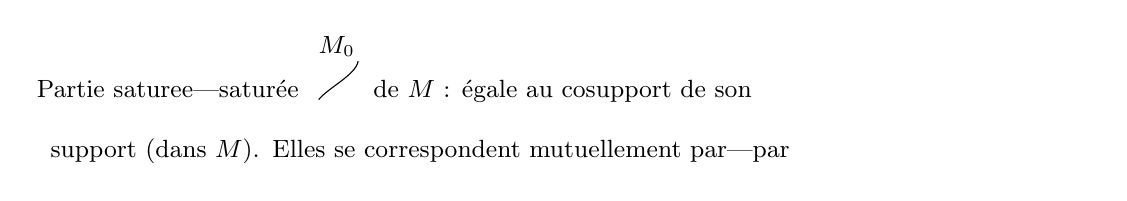
\begin{tikzpicture}[x=1cm,y=1cm,every node/.style={font=\small}]
\node[anchor=base east] at (3.4,0) {Partie \unsure{saturee|saturée}};
\node[anchor=base] at (3.76,.55) {$\inserted{M_0}$};
\draw (4.03,.46) .. controls (4.01,.29) and (3.65,.12) .. (3.53,-.03);
\node[anchor=base west] at (4.1,0) {de $M$ : égale au cosupport de son};
\node[anchor=north west,text width=13.2cm] at (0,-.4)
  {support (dans $M$). Elles se correspondent \unsure{mutuellement} \unsure{par|\deleted{par}}};
\end{tikzpicture}%
}
\[
\begin{aligned}
M_0&=\mathcal F_0\cap M\\
\mathcal F_0&=\{\,F\in\mathcal F\mid\overline F\subset M_0\,\}
\end{aligned}
\]

\scanpage{68}\mspage{67}
\deleted{On a une notion de \unsure{``c|``C|``6}}

Toute partie de $\mathcal F$ (resp $M$) est contenue dans une partie saturée \unsure{minimale} (parmi \unsure{telles|celles} la contenant) qui \deleted{s'appelle \unsure{du|de}} n'est autre que le cosupport du cosupport, et s'appelle aussi son support. Les parties saturées sont celles qui sont égales au support, ou au cosupport, d'une partie. L'application . $\operatorname{cosup}$ \unsure{definit|définit} une \unsure{bij\inserted{e}ction} de l'ens des parties \unsure{saturées|saturée} sur elles $=$, renversant la relation d'inclusion.

On désigne par $\Sigma$ l'ens des \uline{supports} \uline{virtuels}, ou parties saturées
% Figure R1-F1: raised M_0 and its curved oblique insertion leader, without arrowhead.
\figure{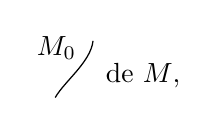
\begin{tikzpicture}[x=1cm,y=1cm]
  \node[anchor=base west] at (0,0) {de $M$,};
  \node[anchor=base east] at (-0.13,0.34) {$\inserted{M_0}$};
  \draw[line width=0.45pt] (-0.52,-0.19) .. controls (-0.40,0.02) and (-0.07,0.26) .. (-0.04,0.53);
\end{tikzpicture}}
où \deleted{\unsure{de}} $\mathcal F_0$ de $M$. \deleted{On \unsure{définit}} \deleted{L'application de cosupport \unsure{d|de}} On \unsure{désidentifie} $\Sigma$ de \deleted{$\unsure{\mathscr P|\mathcal F_2|\mathcal F_0|\mathcal F}$} ses deux 
% Two detached points beneath the word, with no inferred function.
\figure{%
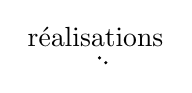
\begin{tikzpicture}[x=1cm,y=1cm]
\node[anchor=base west,inner sep=0] at (0,0) {\unsure{réalisations}};
\fill (0.92,-0.14) circle[radius=0.022cm];
\fill (1.00,-0.20) circle[radius=0.022cm];
\end{tikzpicture}%
}
 (comme \unsure{partie|parties} de $\unsure{P|\mathscr P|\mathcal P}(M)$, ou de $\mathscr P(\unsure{\mathcal F|F})$) et on écrit, pour $\sigma\in\Sigma$
\[
M_\sigma\subset M,\qquad\mathcal F_\sigma\subset\unsure{\mathcal F|F}
\]

Dans $\Sigma$, \deleted{pour} la notion de cosupport est une anti\unsure{\deleted{invo}lution|involution|bijection|dualité} d'ens. ordonnés. Dans $\Sigma$, on a des $\mathrm{Inf}$ quelconques (c'est l'intersection des parties de $M$, ou de $\mathcal F$), et des $\mathrm{Sup}$ quelconques (c'est la partie saturée

\scanpage{69}\mspage{68}
% First paragraph; the two additions and their distinct connecting strokes are kept in this local group.
% figure R1-F1
\figure{%
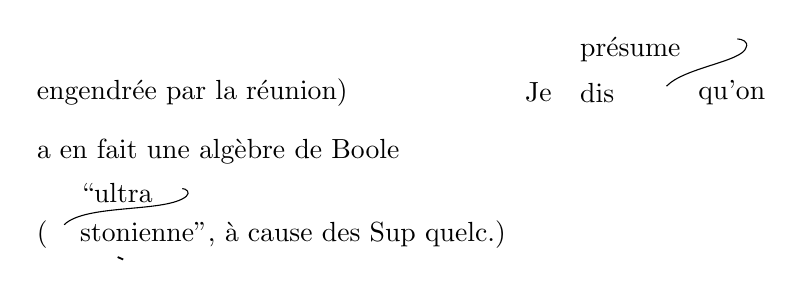
\begin{tikzpicture}[x=1cm,y=1cm]
  \node[anchor=west] at (0,1.8) {engendrée par la réunion)};
  \node[anchor=west] at (6.2,1.8) {Je};
  \node[anchor=west] at (6.9,1.8) {\deleted{dis}};
  \node[anchor=west] at (8.4,1.8) {qu'on};
  \node[anchor=west] at (6.9,2.35) {\inserted{présume}};
  \draw (8.12,1.88) .. controls (8.35,2.12) and (9.08,2.19) .. (9.13,2.37) .. controls (9.17,2.45) and (9.07,2.48) .. (9.02,2.48);
  \node[anchor=west] at (0,1.05) {a en fait une algèbre de Boole};
  \node[anchor=west] at (0,0) {(};
  \node[anchor=west] at (0.55,0) {stonienne'', à cause des $\mathrm{Sup}$ quelc.)};
  \node[anchor=west] at (0.55,0.53) {\inserted{``ultra}};
% Detached short stroke below stonienne; no function is assigned.
  \draw[line width=0.65pt] (1.15,-0.29)--(1.22,-0.32);
  \draw (0.47,0.12) .. controls (0.74,0.39) and (1.76,0.27) .. (2.02,0.48) .. controls (2.08,0.53) and (2.02,0.58) .. (1.97,0.58);
\end{tikzpicture}%
}
% slanted left margin note
\margin{Cela sera valable dans ``le cas ensembliste'', et en tous cas dans les exemples types, donnés \deleted{\unsure{tout}} au début, en termes d'un $E$ (top. ou mesurable), alors $\Sigma$ s'identifie à l'ens des parties de $E$, et \unsure{on trouve|on trouvera|on retrouve} le compactifié de \unsure{Stone} de $E_{\mathrm{disc.}}$ Dans le cas qui vient, \unsure{je} \unsure{ne vois} comment \unsure{prouver}, pour trois supports
\[P,Q,R\quad P\wedge(Q\vee R)=\unsure{\{|(}(P\wedge Q)\vee(P\wedge R)\unsure{\}|.|,|)}\]}

\deleted{Il faudra y revenir}

\unsure{Donc} les supports \unsure{s'identifient|s'identifieraient} aux \unsure{Parties|Partie} à la fois ouvertes et fermées du spectre, qui serait un espace \deleted{\unsure{to|tot}}\unsure{cpct|cpt|compact} \deleted{\unsure{tot}} \unsure{disconnexe} ultra.stonien.

L'involution correspond au passage au complémentaire.

% Construction paragraph with the two insertion leaders; words occur once.
% figure R1-F2
\figure{%
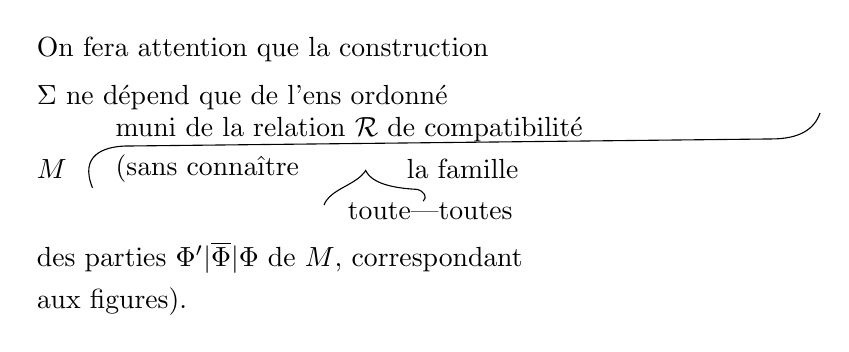
\begin{tikzpicture}[x=1cm,y=1cm]
  \node[anchor=west] at (0,2.0) {On \unsure{fera} attention que la construction};
  \node[anchor=west] at (0,1.38) {$\Sigma$ ne dépend que de l'ens ordonné};
  \node[anchor=west] at (0,0.48) {$M$};
  \node[anchor=west] at (1.0,0.48) {(sans connaître};
  \node[anchor=west] at (4.7,0.48) {la famille};
  \node[anchor=west] at (1.0,0.98) {\inserted{muni de la relation $\mathcal R$ de compatibilité}};
  \draw (0.83,0.24) .. controls (0.66,0.66) and (0.98,0.76) .. (1.24,0.77) -- (9.45,0.86) .. controls (9.82,0.86) and (10.00,0.99) .. (10.07,1.19);
  \node[anchor=west] at (3.95,-0.06) {\inserted{\unsure{toute|toutes}}};
  \draw (3.77,0.02) .. controls (3.85,0.23) and (4.18,0.27) .. (4.30,0.46) .. controls (4.39,0.26) and (4.77,0.23) .. (4.95,0.22) .. controls (5.04,0.20) and (5.09,0.12) .. (5.03,0.07);
  \node[anchor=west] at (0,-0.65) {des parties $\unsure{\Phi'|\overline\Phi|\Phi}$ de $M$, correspondant};
  \node[anchor=west] at (0,-1.20) {aux figures).};
\end{tikzpicture}%
}
En effet, en termes de $(M,\leq,R)$, le cosupport d'une partie $M'$ de $M$ est défini par
\[
\operatorname{cosup}_M(M')=\{\,x\in M\mid(x,x')\in\mathcal R\quad\forall x'\in\unsure{M'|M''}\,\}
\]
% Slanted bottom margin note and its long attached rule; no arrowhead is supplied.
% figure R1-F3
\figure{%
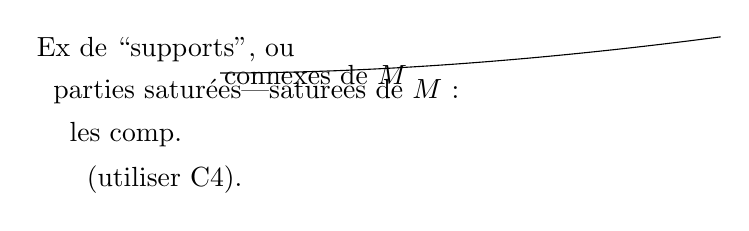
\begin{tikzpicture}[x=1cm,y=1cm]
\begin{scope}[rotate=21]
  \node[anchor=west] at (0,0) {\uline{Ex} de ``supports'', ou};
  \node[anchor=west] at (0,-0.58) {parties \unsure{saturées|saturees} de $M$ :};
  \node[anchor=west] at (0,-1.16) {les comp.};
  \node[anchor=west] at (2.10,-1.16) {connexes de $M$};
  \node[anchor=west] at (0,-1.77) {(utiliser C4).};
  \draw (2.18,-1.16) .. controls (4.23,-1.95) and (6.45,-2.57) .. (8.28,-3.01);
\end{scope}
\end{tikzpicture}%
}

\scanpage{70}\mspage{69}
J'en viens à la rel d'ordre $\preceq$ (subdivision), de nature \unsure{très|trs} différente. Il n'y aura pas de plus petit (ni de plus grand) élément, pas de $\mathrm{Sup}$ de deux \deleted{\unsure{éléments|élémen}}
% G1: local interlinear layout. The long oblique stroke is drawn without an assigned function or an arrowhead; it may meet the initial letter of the following word.
\figure{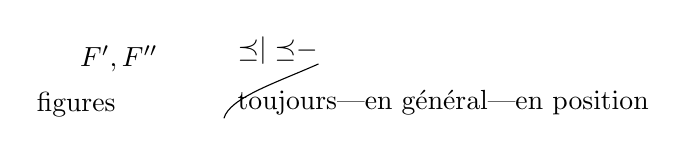
\begin{tikzpicture}[x=1cm,y=1cm]
\node[anchor=base west] at (0,0) {figures};
\node[anchor=base west] at (0.55,0.58) {\inserted{$F',F''$}};
\node[anchor=base west] at (2.55,0.69) {$\inserted{\unsure{\deleted{\preceq}|\preceq}-}$};
\draw (2.50,-0.08) .. controls (2.57,0.18) and (3.16,0.37) .. (3.70,0.61);
\node[anchor=base west] at (2.55,0.03) {\unsure{toujours|en général|en position}};
\end{tikzpicture}}
(i.e. Subdivisions d'une $=$ figure $F$, mais parfois un $\inf$.

On dit que deux subdivision $F',F'''$ de $F$ sont \uline{comp\unsure{\deleted{ati}ara|\deleted{atib}ara|ata|ati}bles} \deleted{\unsure{quand et|on dit} que \unsure{seul|seult|sub|seulement}} (je ne dirai pas ``compatibles'', vu que le terme est déjà pris) si elles admettent une subdivision commune.

% D1: the sole right F is level with the upper F'; the lower-right relation ends in blank space.
% The additional thin upper stroke belongs to the worked upper-right relation; no separate complete older glyph is asserted.
\diagram{\begin{tikzcd}[ampersand replacement=\&,row sep=0.25em,column sep=0.4em]
\& F' \arrow[r,phantom,"{\text{\unsure{
\begin{tikzpicture}[baseline=-0.5ex,x=0.32cm,y=0.32cm]
\draw[line width=0.65pt] (0,0.34) .. controls (0.4,0.37) and (0.8,0.45) .. (1.05,0.86);
\draw[line width=0.3pt] (0.05,0.26) .. controls (0.5,0.29) and (1.05,0.58) .. (1.36,0.84);
\draw[line width=0.65pt] (0,0.34) .. controls (0.42,0.38) and (0.92,0.46) .. (1.18,0.12);
\draw[line width=0.65pt] (0.08,0.03) .. controls (0.48,0.16) and (0.95,0.13) .. (1.13,-0.14);
\end{tikzpicture}}}}" description] \& F \\
F''' \arrow[ur,phantom,"\scriptstyle\preceq" description,sloped] \arrow[dr,phantom,"\scriptstyle\preceq" description,sloped] \& \& {} \\
\& F'' \arrow[ur,phantom,"\scriptstyle\preceq" description,sloped] \&
\end{tikzcd}}
% slanted
\margin{On sera amené à renforcer encore cette condition sur les contrées modérées !}

On dit que la \uuline{\unsure{contrée|contrie}} est \uuline{modérée} si deux subdivision \unsure{d'|\deleted{d'}}\unsure{une|un} $=$ $F$ sont toujours comparables. \deleted{Dans le cas qui vient,}
% G3: on a, its two detached points, the cancelled C5 and the opening
% of the properties paragraph retain their relative positions.
\figure{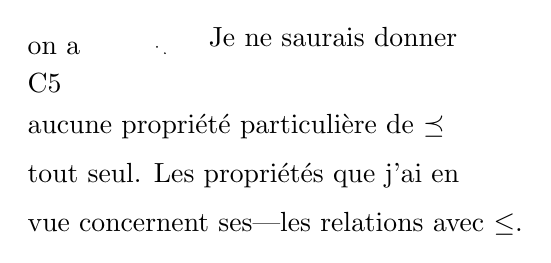
\begin{tikzpicture}[x=1cm,y=1cm]
\node[anchor=base west,inner sep=0pt] at (0,0) {\deleted{on a}};
\fill (1.65,0.10) circle (0.012);
\fill (1.75,0.02) circle (0.012);
\node[anchor=base west,inner sep=0pt] at (2.30,0.10) {Je ne saurais donner};
\node[anchor=base west,inner sep=0pt] at (0,-0.48) {\deleted{\uline{C5}}};
\node[anchor=base west,inner sep=0pt] at (0,-1.00) {aucune propriété particulière de $\preceq$};
\node[anchor=base west,inner sep=0pt] at (0,-1.62) {\deleted{tout} seul. Les propriétés que j'ai en};
\node[anchor=base west,inner sep=0pt] at (0,-2.24) {vue concernent \unsure{ses|les} relations avec $\leq$.};
\end{tikzpicture}}

% slanted
\margin{\unsure{Reporter|reporter} après C6, $C7_0$ ces axiomes \uline{de disjonction}}
% G4: the two long marks stand to the left of the live C5 axiom.
\figure{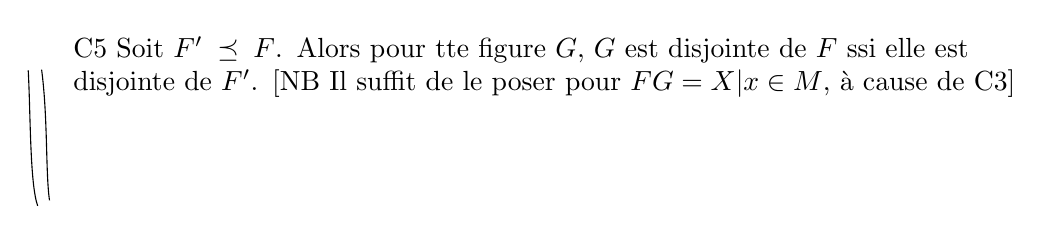
\begin{tikzpicture}[x=1cm,y=1cm]
\draw (0,0) .. controls (0.03,-0.55) and (0.02,-1.44) .. (0.12,-1.72);
\draw (0.17,0.01) .. controls (0.25,-0.60) and (0.22,-1.30) .. (0.27,-1.65);
\node[anchor=north west,text width=12cm,align=left] at (0.45,0.55) {\uline{C5} Soit $F'\preceq F$. Alors pour tte figure $G$, $G$ est disjointe de $F$ ssi elle est disjointe de $F'$. [\uline{NB} Il suffit de le poser pour $\deleted{\unsure{F}}G=\unsure{X|x}\in M$, à cause de C3]};
\end{tikzpicture}}

\scanpage{71}
\mspage{\deleted{\unsure{69|79}}\unsure{70|79}}

Il revient au $=$ de dire que $F$ et $F'$ ont $=$ cosupport, ou encore, même support.

\unsure{Donnons nous} un support.

% G1 margin-mark columns: the two disconnected groups are drawn, without assigning them a linguistic function.
\figure{
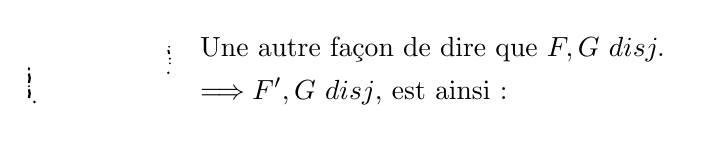
\begin{tikzpicture}[x=1cm,y=1cm]
  \node[anchor=north west,align=left] at (2.15,0.55) {Une autre façon de dire que $F,G\ \text{disj.}$\\[0.35em]
  $\Longrightarrow F',G\ \text{disj}$, est ainsi :};
  \fill (0.10,0.02) ellipse (0.016 and 0.024);
  \draw[line width=0.8pt] (0.10,-0.04)--(0.11,-0.10)--(0.10,-0.16);
  \fill (0.10,-0.20) circle (0.014);
  \draw[line width=0.8pt] (0.10,-0.24)--(0.11,-0.29)--(0.10,-0.35);
  \fill (0.17,-0.40) circle (0.018);
  \fill (1.88,0.30) circle (0.013);
  \draw[line width=0.7pt] (1.87,0.26)--(1.88,0.21);
  \fill (1.89,0.15) circle (0.015);
  \fill (1.89,0.09) circle (0.013);
  \fill (1.87,-0.03) circle (0.017);
\end{tikzpicture}}

% G2: the long rising stroke crosses de beneath the raised addition; deletion versus a crossing insertion arm remains uncertain.
\figure{
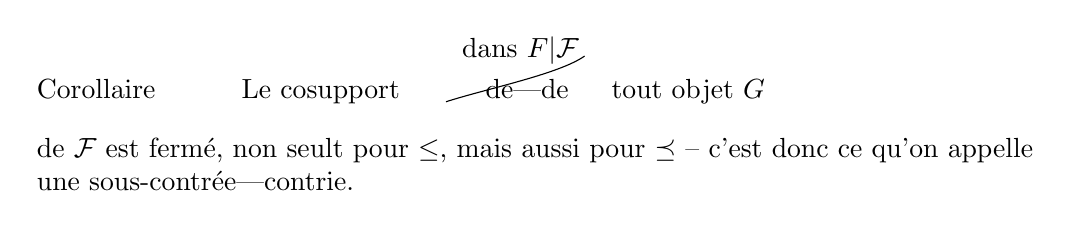
\begin{tikzpicture}[x=1cm,y=1cm]
  \node[anchor=base west] at (0,0) {\uline{Corollaire}};
  \node[anchor=base west] at (2.60,0) {Le cosupport};
  \node[anchor=base west] at (5.70,0) {\unsure{\deleted{de}|de}};
  \node[anchor=base west] at (5.40,0.52) {\inserted{dans $\unsure{F|\mathcal F}$}};
  \draw (5.32,-0.04) .. controls (5.85,0.13) and (6.75,0.31) .. (7.08,0.54);
  \node[anchor=base west] at (7.30,0) {tout objet $G$};
  \node[anchor=north west,text width=12.7cm,align=left] at (0,-0.38) {de $\mathcal F$ est fermé, non seult pour $\leq$, mais aussi pour $\preceq$ -- c'est donc ce qu'on appelle une \uline{sous}-\unsure{contrée|contrie}.};
\end{tikzpicture}}

% G3 itou high mark: the final detached high stroke is reproduced; its role in the word is uncertain.
\figure{

\begin{tikzpicture}[x=1cm,y=1cm]
  \node[anchor=base west] at (0,0) {Donc};
  \node[anchor=base west] at (1.15,0) {\unsure{itou}};
  \draw (1.91,0.33)--(1.96,0.49)--(2.03,0.38);
  \node[anchor=base west] at (3.45,0) {pour toute partie $\Phi\subset\mathcal F$.};
\end{tikzpicture}}

% G4 right punctuation: the punctuation after leq is drawn in place. The loop and short right arm meet the sheet edge.
\figure{
\begin{tikzpicture}[x=1cm,y=1cm]
  \node[anchor=base west] at (0,0) {En d'autres termes, \deleted{toute} partie};
  \node[anchor=base west] at (0,-0.58) {de $\mathcal F$ qui est un $\mathcal F$-support (ou};
  \node[anchor=base west] at (0,-1.16) {``$\mathcal F$-\unsure{saturee|saturée}, sous-entendu : en termes de $\leq$};
  \node[anchor=base west] at (12.05,-1.16) {\unsure{\begin{tikzpicture}[x=1cm,y=1cm,baseline=0pt]
    \draw[line width=0.6pt] (0.04,0.01) .. controls (0.09,-0.09) and (0.04,-0.17) .. (-0.02,-0.20);
    \draw (0.16,0.36) .. controls (0.43,0.10) and (0.43,-0.10) .. (0.23,-0.23);
    \draw (0.30,0.22) .. controls (0.33,0.26) and (0.38,0.18) .. (0.45,0.17) .. controls (0.54,0.15) and (0.41,0.08) .. (0.35,0.04);
    \draw (0.37,0.02)--(0.54,-0.02);
  \end{tikzpicture}}};
  \node[anchor=base west] at (0,-1.85) {cf \unsure{pg|page|pge} $67$) est \unsure{automatiquemt|automatiquement} \deleted{\unsure{f}}une};
  \node[anchor=base west] at (0,-2.43) {sous-contrée.};
\end{tikzpicture}}

% The following two-position folio and draft are upside down on the sheet.
% The second numeral is overwritten; the broad cancellation strokes start below the folio.
\mspage{5\rlap{\deleted{\unsure{4|3}}}5}

% G5 inverted cancelled draft. Text occurs once, in the same group as the boundary and oblique cancellation strokes.
% The isolated glyph under the first Phi is not securely separable from its retracing.
\figure{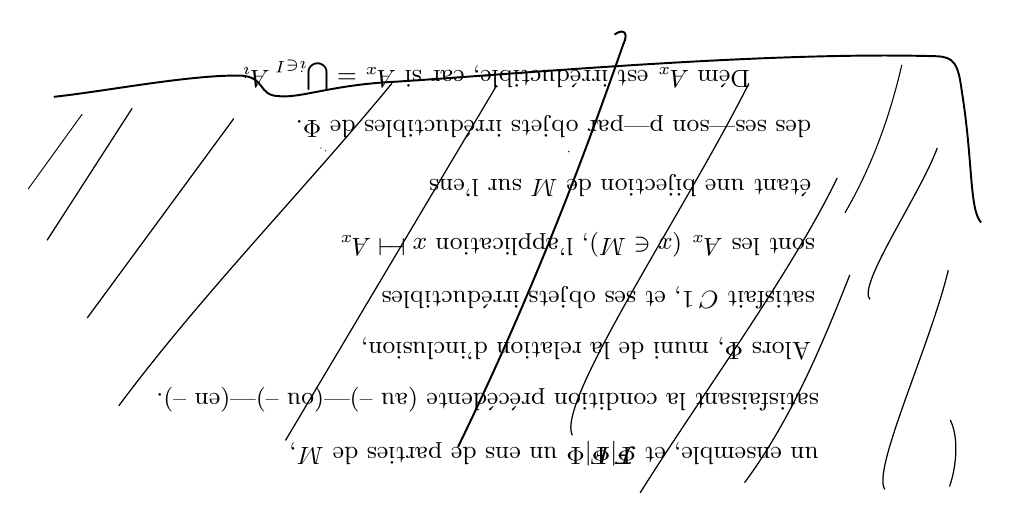
\begin{tikzpicture}[x=0.005cm,y=-0.005cm,font=\small]
\begin{scope}[rotate=180,transform shape]
\node[anchor=base west,inner sep=0pt] at (410,220) {\deleted{un ensemble, et $\unsure{\rlap{\ensuremath{\deleted{\mathcal F}}}\Phi|\rlap{\ensuremath{\deleted{F}}}\Phi|\Phi}$ un ens de parties de $M$,}};
\node[anchor=base west,inner sep=0pt] at (410,355) {\deleted{satisfaisant la condition précédente \unsure{(au --)|(ou --)|(en --)}.}};
\node[anchor=base west,inner sep=0pt] at (430,485) {\deleted{Alors $\Phi$, muni de la relation d'inclusion,}};
\node[anchor=base west,inner sep=0pt] at (420,615) {\deleted{satisfait $C\,1$, et ses objets irréductibles}};
\node[anchor=base west,inner sep=0pt] at (420,750) {\deleted{sont les $A_x$ $(x\in M)$, l'application $x\mathrel{\vdash\joinrel\dashv} A_x$}};
\node[anchor=base west,inner sep=0pt] at (430,900) {\deleted{étant une bijection de $M$ sur l'ens}};
\node[anchor=base west,inner sep=0pt] at (430,1050) {\deleted{des \deleted{\unsure{ses|son}} \deleted{\unsure{p|par}} objets irréductibles de $\Phi$.}};
\node[anchor=base west,inner sep=0pt] at (585,1177) {\deleted{Dém $A_x$ est irréductible, car si $A_x=\bigcup_{i\in I} A_i$}};
% One detached high point after the second inner cancellation, and two low points beneath irreductibles.
\fill (1046,970) circle (2.0);
\fill (1663,972) circle (1.7);
\fill (1675,979) circle (1.7);
% The boundary is open at the scan edge; its upper continuation is not inferred.
\draw[line width=0.7pt] (0,790) .. controls (30,825) and (20,945) .. (49,1125)
 .. controls (58,1195) and (70,1210) .. (112,1212)
 .. controls (550,1225) and (1200,1165) .. (1492,1147)
 .. controls (1650,1139) and (1730,1104) .. (1784,1111)
 .. controls (1835,1113) and (1815,1159) .. (1878,1163)
 .. controls (2010,1165) and (2215,1124) .. (2353,1109);
% Thirteen distinct oblique or curved cancellation strokes.
\draw[line width=0.45pt] (80,120) .. controls (62,170) and (56,245) .. (78,289);
\draw[line width=0.45pt] (244,113) .. controls (278,160) and (130,475) .. (83,669);
\draw[line width=0.45pt] (282,595) .. controls (315,630) and (155,860) .. (111,979);
\draw[line width=0.45pt] (600,130) .. controls (485,285) and (405,474) .. (333,657);
\draw[line width=0.45pt] (865,104) .. controls (720,336) and (480,664) .. (365,903);
\draw[line width=0.40pt] (345,815) .. controls (276,934) and (231,1060) .. (201,1190);
\draw[line width=0.45pt] (1037,250) .. controls (1080,332) and (758,808) .. (589,1143);
\draw[line width=0.72pt] (1327,221) .. controls (1130,625) and (993,997) .. (908,1242)
 .. controls (892,1275) and (910,1282) .. (930,1267);
\draw[line width=0.45pt] (1765,237) -- (1229,1138);
\draw[line width=0.45pt] (2188,325) .. controls (1978,607) and (1714,877) .. (1495,1143);
\draw[line width=0.45pt] (2268,548) -- (1896,1054);
\draw[line width=0.45pt] (2370,745) -- (2154,1080);
\draw[line width=0.35pt] (2418,875) -- (2281,1065);
\end{scope}
\end{tikzpicture}}

\scanpage{72}\mspage{71}

Pour la suite, il faut faire attention si les axiomes vont passer aux sous-contrées. Introduisons quand $= =$ la définition en forme

% fig-definition: the raised word and its full hooked connector, with adjoining text once.
\figure{\begin{tikzpicture}[x=1cm,y=1cm]
\node[anchor=west] at (0,0) {\uline{Définition 1} On appelle};
\node[anchor=west] at (7.4,0) {\uline{sous-contrée}};
\node[anchor=west] at (9.4,0.8) {\inserted{[\uline{pleine}]}};
\draw[line width=.55pt] (8.45,.48) .. controls (8.0,.28) and (10.9,.22) .. (11.35,.1) .. controls (11.85,.02) and (11.9,-.12) .. (12.0,-.23) .. controls (12.17,.03) and (12.28,.37) .. (12.31,.55);
\node[anchor=west] at (0,-1.05) {de la contrée $\unsure{\rlap{$\deleted{\mathcal F}$}\mathcal C|\mathcal C|\mathscr C|\mathbb C}=(\mathcal F,\leq,\preceq)$, \unsure{tout|\deleted{tout}}};
\node[anchor=west] at (0,-1.85) {sous-ens. qui \unsure{satisfont|satisfait} les conditions};
\end{tikzpicture}}

% fig-a-insertions: correspond joins the physical line-end hyphen under convention 7; both insertion arms remain.
\figure{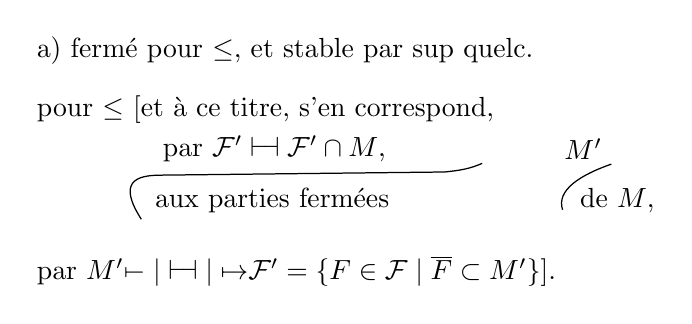
\begin{tikzpicture}[x=1cm,y=1cm]
\node[anchor=west] at (0,0) {a) fermé pour $\leq$, et stable par sup quelc.};
\node[anchor=west] at (0,-.75) {pour $\leq$ [et à ce titre, s'en correspond,};
\node[anchor=west] at (1.5,-1.9) {aux parties fermées};
\node[anchor=west] at (6.9,-1.9) {de $M$,};
\node[anchor=west] at (1.6,-1.25) {\inserted{par $\mathcal F'\mathrel{\vdash\joinrel\dashv}\mathcal F'\cap M$,}};
\node[anchor=west] at (6.7,-1.25) {\inserted{$M'$}};
\draw[line width=.45pt] (1.45,-2.14) .. controls (1.15,-1.67) and (1.37,-1.58) .. (1.7,-1.58) -- (5.3,-1.54) .. controls (5.5,-1.52) and (5.62,-1.50) .. (5.78,-1.43);
\draw[line width=.45pt] (6.8,-2.02) .. controls (6.72,-1.77) and (7.02,-1.58) .. (7.42,-1.44);
\node[anchor=west] at (0,-2.8) {par $M'\unsure{\mathrel{\mapstochar\relbar}|\mathrel{\vdash\joinrel\dashv}|\mapsto}\mathcal F'=\{F\in\mathcal F\mid\overline F\subset M'\}$].};
\end{tikzpicture}}

% slanted left margin; the terminal close is covered by root crop a05.
\margin{Je ne sais s'il faut prendre des sup quelconques (\unsure{condition} stricte) \deleted{\unsure{et}} ou bien de sup finis seulement \unsure{(condition lge)|(condition large)}}

% fig-b-correction: replacement above the cancelled clause; crossed/curling mark after M.
\figure{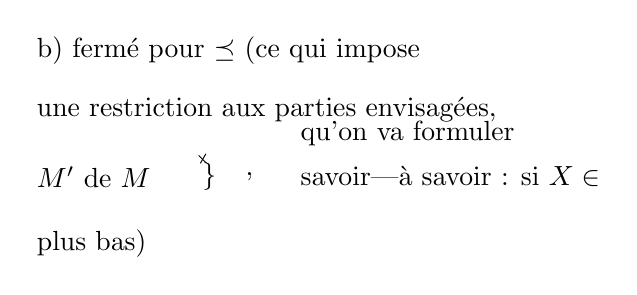
\begin{tikzpicture}[x=1cm,y=1cm]
\node[anchor=west] at (0,0) {b) fermé pour $\preceq$ (ce qui impose};
\node[anchor=west] at (0,-.75) {une restriction aux parties envisagées,};
\node[anchor=west] at (0,-1.6) {$M'$ de $M$};
% fig-b-curled-mark: curled stroke with a small crossing at its head.
\node[anchor=west] at (2.1,-1.6) {\unsure{\}}};
\draw[line width=.35pt] (2.18,-1.33) -- (2.28,-1.43);
\draw[line width=.35pt] (2.20,-1.43) -- (2.27,-1.31);
\node[anchor=west] at (2.65,-1.6) {,};
\node[anchor=west] at (3.35,-1.6) {\deleted{\unsure{savoir|à savoir} : si $X\in$}};
\node[anchor=west] at (3.35,-1.05) {\inserted{qu'on va formuler}};
\node[anchor=west] at (0,-2.45) {plus bas)};
\end{tikzpicture}}

% fig-marginal-c: marginal continuation above C6; labels occur only here.
\figure{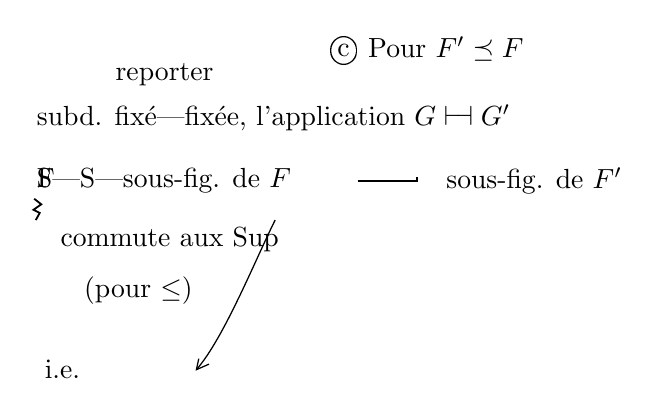
\begin{tikzpicture}[x=1cm,y=1cm]
\node[anchor=west] at (1.0,.55) {reporter};
\node[anchor=west] at (3.7,.85) {\textcircled{c} Pour $F'\preceq F$};
\node[anchor=west] at (0,0) {subd. \unsure{fixé|fixée}, l'application $G\mathrel{\vdash\joinrel\dashv}G'$};
% The worked initial is ONE letter position, including the lower residual strokes.
\node[anchor=west] at (0,-.8) {\unsure{\rlap{\deleted{F}}S|S|s}ous-fig. de $F$};
\draw[line width=.65pt] (.09,-1.03) -- (.18,-1.10) -- (.08,-1.17) -- (.16,-1.21) -- (.11,-1.30);
% fig-c-headless-link: horizontal stroke with a very short raised right endpoint, no arrowhead.
\draw[line width=.6pt] (4.2,-.8) -- (4.95,-.8) -- (4.95,-.75);
\node[anchor=west] at (5.2,-.8) {sous-fig. de $F'$};
\node[anchor=west] at (.3,-1.55) {commute aux Sup};
\node[anchor=west] at (.6,-2.2) {(pour $\leq$)};
\node[anchor=west] at (.1,-3.2) {i.e.};
% A distinct pointer descends leftward from the aux region.
\draw[line width=.45pt] (3.15,-1.3) .. controls (2.9,-1.8) and (2.5,-2.8) .. (2.15,-3.2);
\draw[line width=.45pt] (2.18,-3.06) -- (2.15,-3.2) -- (2.31,-3.13);
\end{tikzpicture}}

% diagram: C6-group. Diagrams remain diagrams; the two side rules, detached
% points and oblique gloss keep their relative positions. No text is repeated.
\diagram{\begin{tikzpicture}[x=1cm,y=1cm]
\node[anchor=west] at (0,0) {\uline{C6}};
\node[anchor=west] at (2.15,0) {Soit};
\node at (4.05,-1.45) {\begin{tikzcd}[ampersand replacement=\&,column sep=1.6em,row sep=1.5em]
F' \arrow[r,phantom,"{\preceq}" description] \& F \arrow[d,phantom,"{\rotatebox{90}{$\leq$}}" description] \\
\& G
\end{tikzcd}};
\node[anchor=west] at (7.90,-1.15) {de $\mathcal F$};
\fill (2.01,-.88) circle (.012);
\fill (2.08,-.93) circle (.012);
\draw[line width=.4pt] (-.30,-.18) .. controls (-.27,-1.92) and (-.34,-3.62) .. (-.19,-4.78);
% slanted; the long rule is not treated as cancellation of this gloss.
\node[anchor=west,rotate=44,align=left] at (-2.00,-2.25) {sym\unsure{e|é}trique\\en $\leq,\preceq$};
\fill (-.46,-2.12) circle (.012);
\node[anchor=west] at (0,-3.05) {\textcircled{a} Alors il existe un unique $H\in\mathcal F$ \unsure{avec|ou}};
\node at (4.10,-4.86) {\begin{tikzcd}[ampersand replacement=\&,column sep=1.6em,row sep=1.5em]
F' \arrow[r,phantom,"{\preceq}" description] \arrow[d,phantom,"{\rotatebox{90}{$\leq$}}" description] \& F \arrow[d,phantom,"{\rotatebox{90}{$\leq$}}" description] \\
G' \arrow[r,phantom,"{\preceq}" description] \& G
\end{tikzcd}};
\node[anchor=west] at (7.05,-3.73) {et};
\node at (7.72,-3.42) {\textcircled{b}};
\node[anchor=west] at (8.04,-3.73) {les \unsure{str.tes|strates} de};
\node[anchor=west] at (7.05,-4.24) {$G'$ sont les \unsure{\deleted{S}|S|s}tr\unsure{a|.}tes};
\node[anchor=west] at (7.05,-4.75) {$X'$ de $F'$ \unsure{tel|\deleted{tel}}les que};
\node[anchor=west] at (7.38,-5.25) {$X'\ll\unsure{G_n|G_m|G}$.};
\node[anchor=west] at (7.28,-5.72) {Ce compl\unsure{\.{e}|é|e}ment servira};
\node[anchor=west] at (7.48,-6.08) {plus bas};
\draw[line width=.5pt] (6.88,-3.67) -- (6.92,-5.70);
\draw[line width=.5pt] (6.98,-3.64) -- (7.02,-5.77);
\draw[line width=.45pt] (6.87,-5.39) -- (7.02,-5.72);
\draw[line width=.45pt] (6.88,-5.49) -- (7.06,-5.47);
\end{tikzpicture}}

On dit que $\unsure{G|\rlap{$\deleted{F}$}G|E}'$ est la \uline{subd} \uline{de} $G$ induite
% figure: bottom-punctuation. The slant, loop and second small curve following
% F are preserved without deciding that they are one or two commas.
\figure{\begin{tikzpicture}[x=1cm,y=1cm]
\node[anchor=west] at (0,0) {par la subd $F'$ de $F$};
\node[anchor=west] at (4.08,.02) {\unsure{\begin{tikzpicture}[x=1cm,y=1cm,baseline=-.1cm]
\draw[line width=.4pt] (.21,.30) -- (.01,-.26) .. controls (-.04,-.42) and (.11,-.42) .. (.10,-.28) .. controls (.06,-.20) and (-.01,-.22) .. (.01,-.26);
\draw[line width=.4pt] (.29,-.24) .. controls (.29,-.34) and (.23,-.39) .. (.18,-.42);
\end{tikzpicture}}};
\node[anchor=west] at (4.75,0) {ou que $G'$ est la \deleted{\unsure{sous-fig|sous-fig.}}};
\end{tikzpicture}}
% slanted
\margin{sur la sous-figure $\unsure{\rlap{$\deleted{F}$}G|G|E}$ de $F$}
